\section{Prefix-free graphs}
% some intro?
The idea of prefix-free graphs is inspired by rsync \cite{kornblum2006identifying}.
%% Context-triggered piecewise hashing (CTPH) is a technique for parsing
%% strings into blocks such that long repeated substrings are parsed the same
%% way (except possibly at the beginning or end of the substrings).

% what are prefix-free graphs
Given a set of sequences representing a pangenome, we can partition each
sequence into \emph{segment}s.
These segments form nodes of the prefix-free graph.
The edges of a graph represent the adjacencies of the segment pairs, which are 
present in the original strings.
The adjacent segments are overlapping by a fixed number of characters $k$.
We will call these $k$-sized overlaps triggers.
Another important feature of the segments is that they contain triggers only at
the start or at the end of a segment.
This feature guarantees that the set of segments is prefix-free, i.e. no
segment is a prefix of another segment.

\begin{figure}
    \centering
    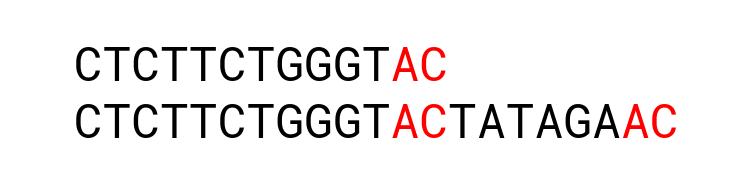
\includegraphics[width=\linewidth]{images/prefixfree_proof.png}
    \caption{Visual proof that the trigger words induce prefix-free segments.}
    \label{fig:proof}
\end{figure}

% how to construct prefix free graphs
To illustrate how to partition the sequences into segments consider a set of
strings $S = {TACTACGTACT, TCGTACTACT, TCGTCGTACTACT}$.
Next, assume we will partition the sequences using a set of trigger words 
$T = {AC, CG}$.

In stringology, strings are often flanked by so called \emph{sentinel} = $\$$.
In our case, we need to append $k$ sentinels to the sequences.
The reasons for doing so will become clear in the suffix array construction section.

Then, using a sliding window we can scan through the sequences and each time we
encounter a trigger word, we create a new segment from the start of the previous
trigger word to the end of the current trigger word.
Two special cases happen at the beginning of a sequence, when no previous
trigger was encountered, and at the end.
In the former case, the segment starts simply at the start of a sequence and in
the later case the segment ends at a sequence end.

During the sequence scan, each unique segment is assigned an ID.
The original sequence can then be represented as a list of IDs, also called 
\emph{path}s.

The result of this procedure is a set of segments and a list of paths.
In the previous example, the segments are ${ TAC, ACTAC, ACG, CGTAC, ACT\$\$, TCG, CGTCG }$
and the paths are $[  ]$.

Because each segment is represented in a set $S$ only once, the sum of lengths
of segments is usually much smaller than the length of original sequences.

This set of segments, together with the list of paths are already a prefix-free
graph, but in order to be useful for the next part, we need to normalize it.
By normalizing, we mean to sort the segments lexicographically and relabel the
paths accordingly.
This will give us a list of segments and a list of paths which can be directly
represented in the GFA format as shown in the Figure \ref{fig:gfa}.

\begin{figure}
    \centering
    % 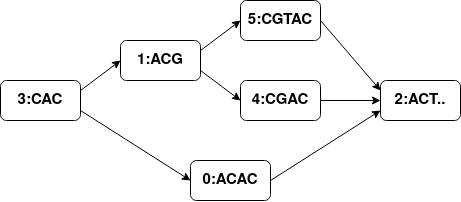
\includegraphics[width=\linewidth]{images/pfg.drawio.png}
    % 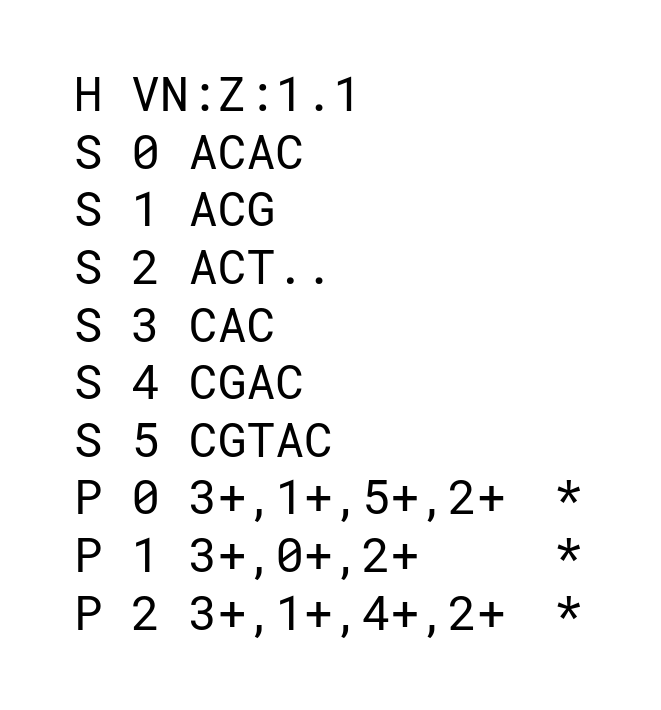
\includegraphics[width=0.5\linewidth]{images/pfg_gfa.v2.png}
    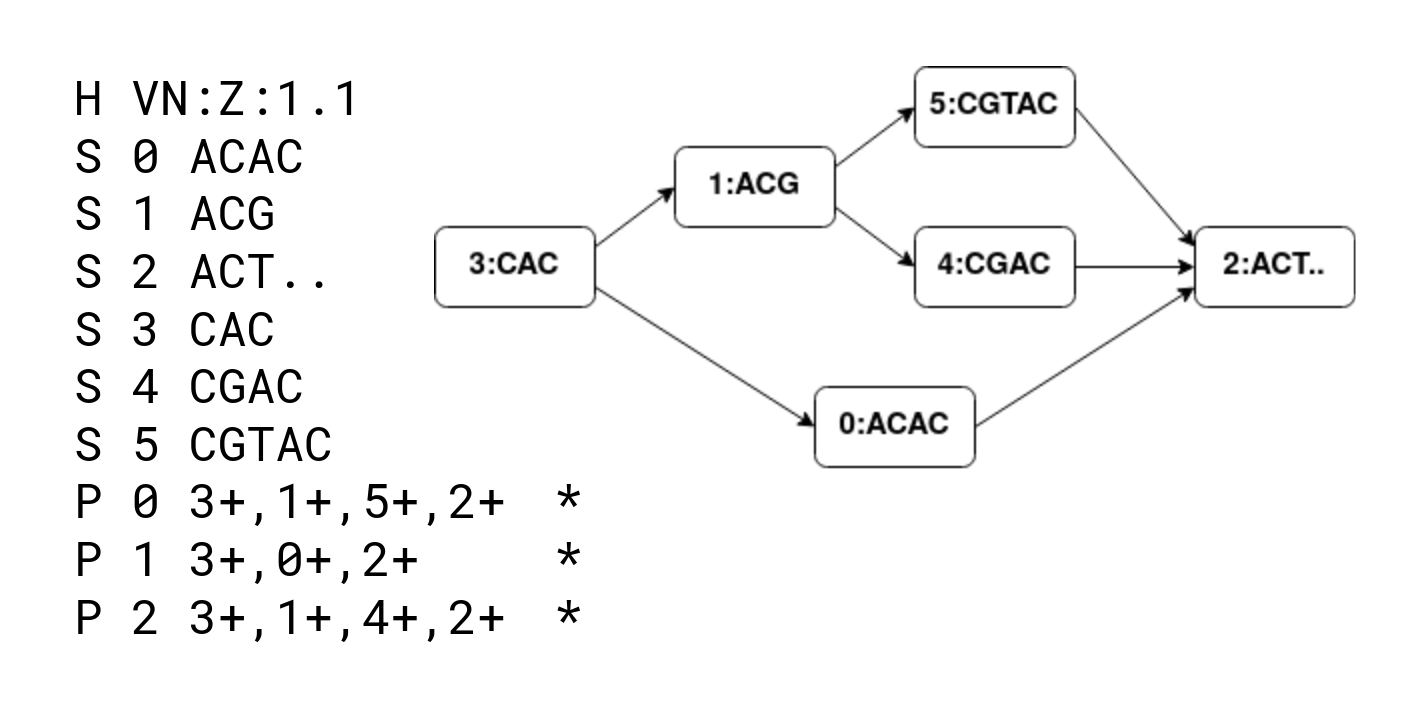
\includegraphics[width=\linewidth]{images/pfg_gfa.v3.png}
    \caption{Prefix-free graph in GFA format. Link lines omitted for brevity.}
    \label{fig:gfa}
\end{figure}

% add graph figure

The reconstruction of the original sequence can then be done by expanding 
the particular path, ignoring last $k$ characters of each segment.


